\documentclass{article}
\usepackage[utf8]{inputenc}
\usepackage{graphicx}
\title{Aerodynamics and Space Systems Design}
\author{Rohil Sheth}
\date{September 2018}
\begin{document}
    \maketitle
    \tableofcontents
    \section{Aircraft Performance}
    \subsection{Forces on an Aircraft}
    \subsubsection{Types of Forces}
    The forces acting on an aircraft can be separated into:
    \begin{enumerate}
        \item Gravitational: The gravitational force is the aircraft’s weight, including all of its contents (i.e.
        fuel, payload, passengers, etc.). Denoted as W.
        \item Propulsive: The propulsive force, referred to as the thrust, is the force acting on the aircraft
        generated by the aircraft’s propulsion system. Denoted as T.
        \item Aerodynamic: The aerodynamic force is defined as the force generated 
        by the air acting on the surface of the aircraft. Denote as A.
        
        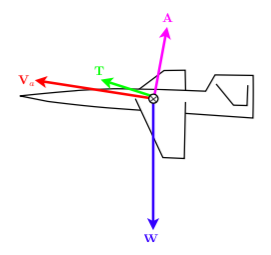
\includegraphics[width=4cm, height=4cm]{forces}

    \end{enumerate}
    \subsubsection{Aerodynamic Forces}
        The aerodynamic force is often decompressed into:
        \begin{itemize}
            \item Drag: The drag, D, is the component of the aerodynamic force acting in the freestream direction.
            \item Lift: The lift, L, is the component of the aerodynamic force acting normal to the freestream direction. In three-dimensional flows, the normal direction is not unique. However, generally, it is an aircraft that is symmetric such that the left and right sides of the aircraft (though control surfaces such as ailerons can break this symmetry) are the same, and the freestream velocity vector is in this plane of symmetry. In this case, the lift is the defined as the force normal to the freestream in the plane of symmetry.
            \item Side: The side force, Y , (also referred to as the yaw force) is the component of the aerodynamic force perpendicular to both the drag and lift directions: it acts along the span-wise direction. Generally, the side force will almost always be zero.
        \end{itemize}
\end{document}